\chapter{Machine Learning}\label{neural-network---practical-lesson-8}

In this Chapter we will see how machine learning techniques can be
successfully applied to solve financial problems. We will first do a
quick tour on the theory behind neural networks and then we will see an
example and two practical applications regarding regression and
classification issues.

This lecture just scratches the surface of the
machine learning topic which has seen a huge development in the latest
years leading to thousands of applications in many different fields.

\section{Neural networks}\label{neural-networks}

Artificial Neural Networks (ANN or simply NN) are information processing
models that are developed by inspiring from the working principles of
human brain. Their most essential property is the ability of learning
from sample sets.

The basic process units of ANN architecture are neurons which are
internally in connection with other neurons.

\begin{figure}
\centering
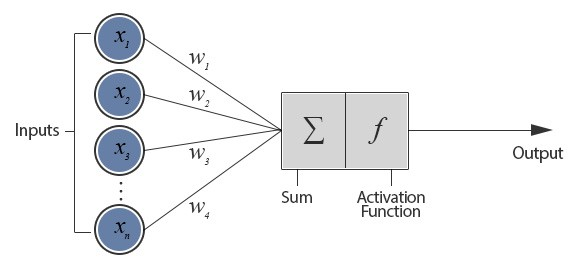
\includegraphics[width=0.8\linewidth]{neuron.jpeg}
\caption{Model of an artificial neuron.}
\end{figure}

A neuron consists of weights (\(w_i\)) and real (\(x_i\)) numbers. All
inputs injected into neurons are individually weighted, added together
and passed into the activation function which produce the neuron output.
There are many different types of activation function but one of the
simplest would be \emph{step function} which returns just 0 or 1
according to the input value (another is the \emph{sigmoid} which can be
thought of as the continuous version of the step function).

\begin{figure}
\centering
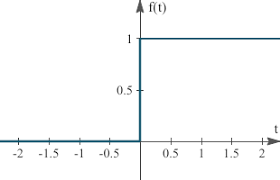
\includegraphics[width=0.4\linewidth]{step_function.png}\quad
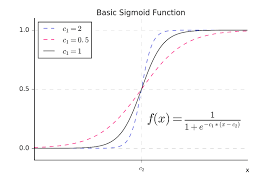
\includegraphics[width=0.4\linewidth]{sigmoid.png}
\caption{On the left an example of step function on the right a sigmoid.}
\end{figure}

\subsection{Training of a neuron}\label{training-of-a-neuron}

When teaching children how to recognize a bus, we just tell them,
showing an example: ``This is a bus. That is not a bus.'' until they
learn the concept of what a bus is. Furthermore, if the child sees new
objects that she hasn't seen before, we could expect her to recognize
correctly whether the new object is a bus or not. This is exactly the
idea behind the neurons. Similarly, inputs from a \emph{training} set
are presented to the neuron one after the other and the neuron weights
are modified according to the expected output.

When an entire pass through all of the input training vectors is
completed the neuron has learnt ! At this time, if an input vector
\(\vec{P}\) (already in the training set) is given to the neuron, it
will output the correct value. If \(\vec{P}\) is not in the training
set, the network will respond with an output similar to other training
vectors close to \(\vec{P}\).

Unfortunately using just a neuron is not too useful since it is not
possible to solve the interesting problems we would like to face with
just that simple architecture. The next step is then to put together
more neurons in \emph{layers}.

\subsection{Multi-layered neural
networks}\label{multi-layered-neural-networks}

\begin{figure}
\centering
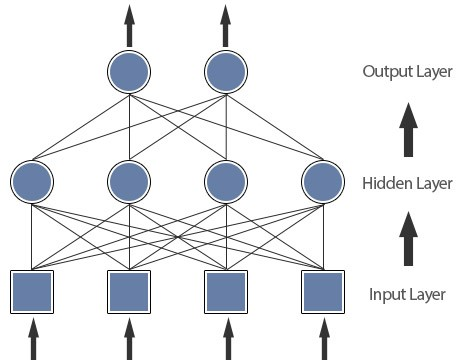
\includegraphics[width=0.7\linewidth]{multilayer.jpeg}
\caption{A multi-layered neural network.}
\end{figure}

Each input from the \emph{input layer} is fed up to each node in the
hidden layer, and from there to each node on the output layer. We should
note that there can be any number of nodes per layer and there are
usually multiple hidden layers to pass through before ultimately
reaching the output layer. But to train this network we need a learning
algorithm which should be able to tune not only the weights between the
output layer and the hidden layer but also the weights between the
hidden layer and the input layer.

\subsection{Back propagation}\label{back-propagation}

In order to tune the weights at each layer at every iteration we should
know what the output would be at each node. But this is not possible
since the only value we know is the correct output at the last node (the
final output of the NN which can be compared to our truth of the
training output). The method that was suggested to overcome the issue
was to take the errors at the output layer (last node) and
proportionally propagate it backwards to all the hidden layer.

So, what it's going to happen is:

\begin{itemize}
\tightlist
\item
  present a training sample to the neural network (initialized with
  random weights);
\item
  compute the output received by calculating activations of each layer
  and thus calculate the error as the difference between the NN output
  and the training sample expected result;
\item
  having calculated the error, readjust the weights such that the error
  (difference) decreases;
\item
  continue the process for all training samples several times until the
  weights are not changing too much (a.k.a. the process converged).
\end{itemize}

The NN error is computed by the \emph{loss function} (usually it is
either the mean squared error or the mean absolute error) and an
\emph{optimization function} is then used to choose the appropriate
weight values in order to reduce the loss function value (we will use
\emph{Adam} as optimizator in the following but there are more).

\subsection{Neural Network Design}\label{neural-network-design}

There is no rule to guide developer into the design of a neural network
in terms of number of layers and neuron per layer. The most common
strategy is a trail and error one where you finally pick up the solution
giving the best accuracy. In general a larger number of nodes is better
to catch highly structured data with a lot of feature although it may
require larger training sample to work correctly.

A common mistake to avoid is to \emph{overtrain} a NN. Overtraining is
what happens when the NN learns too well the training sample but its
performance degrade substantially in an independent testing sample. So
usually it is required to split the available sample in two parts
training and testing (e.g.~80\% and 20\%) and to use the former to
perform the training and the latter to cross-check the performance.
Usually the performance are \emph{measured} with the mean square error
computed between the truth of the sample and the NN predictions.

Anyway as a rule of thumb a NN with just one hidden layer with a number
of neurons averaging the inputs and outputs is sufficient in most cases.
In the following we will use more complex networks just for
illustration, no strong attempt in optimizing the layout has been done
though.

\section{Practical Examples}\label{practical-examples}

Below it will be illustrated few practical applications of neural
network trainings in python. Various modules are available to develop
neural network in \texttt{python}, we will use \texttt{Keras} a
relatively high level library which in turn use \texttt{TensorFlow} a
very famous machine learning tool developed by Google.

In the attempt of keeping things as simple as possible I have added
another layer above \texttt{Keras}, \texttt{FinNN} so that you can try
to design some NN without caring too much about the many details and
parameters that are involved in the process.

\subsection{Function approximation}\label{function-approximation}

As a first practical example let's try to design an ANN which is capable
of learning the functional form underlying a set of data.

Let's generate a sample with \(x\) (input), \(f(x)\) (truth) pairs where
\(f(x) = x^2\) and let's start to code the NN structure.

We start by importing the necessary modules. Then we generate the
training sample (i.e.~the \(x\), \(f(x)\) pairs) and apply a simple
transformation on the sample in order to have all the inputs and outputs
in the \([0, 1]\) range. This is usually done to provide the NN with
\emph{normalized} data, infact the NN can be fooled by large or very
small numbers giving unstable results.

    \begin{tcolorbox}[breakable, size=fbox, boxrule=1pt, pad at break*=1mm,colback=cellbackground, colframe=cellborder]
\begin{Verbatim}[commandchars=\\\{\}]
\PY{k+kn}{from} \PY{n+nn}{finnn} \PY{k}{import} \PY{n}{FinNN}
\PY{k+kn}{from} \PY{n+nn}{numpy} \PY{k}{import} \PY{n}{arange}\PY{p}{,} \PY{n}{asarray}

\PY{c+c1}{\PYZsh{} define the dataset}
\PY{n}{x} \PY{o}{=} \PY{n}{asarray}\PY{p}{(}\PY{p}{[}\PY{n}{i} \PY{k}{for} \PY{n}{i} \PY{o+ow}{in} \PY{n}{arange}\PY{p}{(}\PY{o}{\PYZhy{}}\PY{l+m+mi}{50}\PY{p}{,} \PY{l+m+mi}{50}\PY{p}{,} \PY{l+m+mf}{0.1}\PY{p}{)}\PY{p}{]}\PY{p}{)}

\PY{n}{y} \PY{o}{=} \PY{n}{asarray}\PY{p}{(}\PY{p}{[}\PY{n}{i}\PY{o}{*}\PY{o}{*}\PY{l+m+mf}{2.0} \PY{k}{for} \PY{n}{i} \PY{o+ow}{in} \PY{n}{x}\PY{p}{]}\PY{p}{)}
\PY{n+nb}{print}\PY{p}{(}\PY{l+s+s2}{\PYZdq{}}\PY{l+s+s2}{Distribution of original data }\PY{l+s+s2}{\PYZdq{}}\PY{p}{,} \PY{n}{x}\PY{o}{.}\PY{n}{min}\PY{p}{(}\PY{p}{)}\PY{p}{,} \PY{n}{x}\PY{o}{.}\PY{n}{max}\PY{p}{(}\PY{p}{)}\PY{p}{,} \PY{n}{y}\PY{o}{.}\PY{n}{min}\PY{p}{(}\PY{p}{)}\PY{p}{,} \PY{n}{y}\PY{o}{.}\PY{n}{max}\PY{p}{(}\PY{p}{)}\PY{p}{)}

\PY{n}{trainer} \PY{o}{=} \PY{n}{FinNN}\PY{p}{(}\PY{p}{)}
\PY{n}{trainer}\PY{o}{.}\PY{n}{setData}\PY{p}{(}\PY{n}{x}\PY{p}{,} \PY{n}{y}\PY{p}{)}

\PY{n}{trainer}\PY{o}{.}\PY{n}{normalize}\PY{p}{(}\PY{p}{)}

\PY{c+c1}{\PYZsh{} here you should see that x and y are between 0 and 1}
\PY{n+nb}{print}\PY{p}{(}\PY{l+s+s2}{\PYZdq{}}\PY{l+s+s2}{The same data after the normalization }\PY{l+s+s2}{\PYZdq{}}\PY{p}{,} \PY{n}{trainer}\PY{o}{.}\PY{n}{x}\PY{o}{.}\PY{n}{min}\PY{p}{(}\PY{p}{)}\PY{p}{,} 
      \PY{n}{trainer}\PY{o}{.}\PY{n}{x}\PY{o}{.}\PY{n}{max}\PY{p}{(}\PY{p}{)}\PY{p}{,} \PY{n}{trainer}\PY{o}{.}\PY{n}{y}\PY{o}{.}\PY{n}{min}\PY{p}{(}\PY{p}{)}\PY{p}{,} \PY{n}{trainer}\PY{o}{.}\PY{n}{y}\PY{o}{.}\PY{n}{max}\PY{p}{(}\PY{p}{)}\PY{p}{)}

Using TensorFlow backend.

Distribution of original data  -50.0 49.90000000000143 5.048709793414476e-25
2500.0
The same data after the normalization  0.0 1.0 0.0 1.0
    \end{Verbatim}
\end{tcolorbox}

    Next we can define the structure of the neural network. There is no
predefined rule to decide the number of layers and nodes you need to go
by trial and error. Here the problem is quite simple so there is no need
to use a complicated NN.

In the end I have decided to use two layers with 10 nodes each and a
\emph{sigmoidal} activation function. The input\_dim parameter has to be
set to 1 since we have just one single input, the \(x\) value.

    \begin{tcolorbox}[breakable, size=fbox, boxrule=1pt, pad at break*=1mm,colback=cellbackground, colframe=cellborder]
\begin{Verbatim}[commandchars=\\\{\}]
\PY{c+c1}{\PYZsh{} design the neural network model}
\PY{n}{trainer}\PY{o}{.}\PY{n}{addInputLayer}\PY{p}{(}\PY{l+m+mi}{1}\PY{p}{,} \PY{l+m+mi}{10}\PY{p}{,} \PY{l+s+s1}{\PYZsq{}}\PY{l+s+s1}{sigmoid}\PY{l+s+s1}{\PYZsq{}}\PY{p}{)}
\PY{n}{trainer}\PY{o}{.}\PY{n}{addHiddenLayer}\PY{p}{(}\PY{l+m+mi}{10}\PY{p}{,} \PY{l+s+s1}{\PYZsq{}}\PY{l+s+s1}{sigmoid}\PY{l+s+s1}{\PYZsq{}}\PY{p}{)}
\PY{n}{trainer}\PY{o}{.}\PY{n}{addOutputLayer}\PY{p}{(}\PY{l+m+mi}{1}\PY{p}{)}

\PY{c+c1}{\PYZsh{} define the loss function (mean squared error) and optimization algorithm (Adam)}
\PY{n}{trainer}\PY{o}{.}\PY{n}{compileModel}\PY{p}{(}\PY{l+s+s1}{\PYZsq{}}\PY{l+s+s1}{mse}\PY{l+s+s1}{\PYZsq{}}\PY{p}{,} \PY{l+s+s1}{\PYZsq{}}\PY{l+s+s1}{adam}\PY{l+s+s1}{\PYZsq{}}\PY{p}{)}

\PY{c+c1}{\PYZsh{} fit the model on the training dataset}
\PY{c+c1}{\PYZsh{} using 500 epochs, a batch\PYZus{}size of 10}
\PY{n}{trainer}\PY{o}{.}\PY{n}{fit}\PY{p}{(}\PY{l+m+mi}{500}\PY{p}{,} \PY{l+m+mi}{10}\PY{p}{)}
\end{Verbatim}
\end{tcolorbox}

    After the training is completed we can evaluate how good it is. To do
this we can compute the residuals or the square root of the sum of the
squared difference between the true value and the one predicted by the
NN. We will also plot the true function and the predicted one in order
to have a graphical representation of the goodness of our training. To
have a numerical estimate of the agreement it has been computed also the
\emph{mean squared error} defined as:

\begin{align*}
  MSE = \frac{\sum_{i=1}^n{\big(\frac{x_{i}^{pred} - x_i^{truth}}{x_i^{truth}}\big)^2}}{n}
\end{align*}

A \emph{perfect} prediction would lead to \(MSE=0\) so the lower this
number the better the agreement.

    \begin{tcolorbox}[breakable, size=fbox, boxrule=1pt, pad at break*=1mm,colback=cellbackground, colframe=cellborder]
\begin{Verbatim}[commandchars=\\\{\}]
\PY{k+kn}{from} \PY{n+nn}{sklearn}\PY{n+nn}{.}\PY{n+nn}{metrics} \PY{k}{import} \PY{n}{mean\PYZus{}squared\PYZus{}error}
\PY{k+kn}{from} \PY{n+nn}{matplotlib} \PY{k}{import} \PY{n}{pyplot} \PY{k}{as} \PY{n}{plt}

\PY{c+c1}{\PYZsh{} make predictions for the input data}
\PY{n}{trainer}\PY{o}{.}\PY{n}{fullPrediction}\PY{p}{(}\PY{p}{)}

\PY{c+c1}{\PYZsh{} invert the previous transformation to get back the real data and not the normalized one}
\PY{n}{trainer}\PY{o}{.}\PY{n}{reverseNormalization}\PY{p}{(}\PY{p}{)}

\PY{c+c1}{\PYZsh{} report model error computing the mean squared error}
\PY{n+nb}{print}\PY{p}{(}\PY{l+s+s1}{\PYZsq{}}\PY{l+s+s1}{MSE: }\PY{l+s+si}{\PYZpc{}.3f}\PY{l+s+s1}{\PYZsq{}} \PY{o}{\PYZpc{}} \PY{n}{mean\PYZus{}squared\PYZus{}error}\PY{p}{(}\PY{n}{trainer}\PY{o}{.}\PY{n}{y}\PY{p}{,} \PY{n}{trainer}\PY{o}{.}\PY{n}{predictions}\PY{p}{)}\PY{p}{)}

\PY{c+c1}{\PYZsh{} plot the true function and the prediction to see the actual difference}
\PY{n}{plt}\PY{o}{.}\PY{n}{scatter}\PY{p}{(}\PY{n}{trainer}\PY{o}{.}\PY{n}{x}\PY{p}{,} \PY{n}{trainer}\PY{o}{.}\PY{n}{y}\PY{p}{,} \PY{n}{label}\PY{o}{=}\PY{l+s+s1}{\PYZsq{}}\PY{l+s+s1}{Actual}\PY{l+s+s1}{\PYZsq{}}\PY{p}{)}
\PY{n}{plt}\PY{o}{.}\PY{n}{scatter}\PY{p}{(}\PY{n}{trainer}\PY{o}{.}\PY{n}{x}\PY{p}{,} \PY{n}{trainer}\PY{o}{.}\PY{n}{predictions}\PY{p}{,} \PY{n}{label}\PY{o}{=}\PY{l+s+s1}{\PYZsq{}}\PY{l+s+s1}{Predicted}\PY{l+s+s1}{\PYZsq{}}\PY{p}{,} \PY{n}{s}\PY{o}{=}\PY{l+m+mi}{4}\PY{p}{)}
\PY{n}{plt}\PY{o}{.}\PY{n}{title}\PY{p}{(}\PY{l+s+s1}{\PYZsq{}}\PY{l+s+s1}{Input (x) versus Output (y)}\PY{l+s+s1}{\PYZsq{}}\PY{p}{)}
\PY{n}{plt}\PY{o}{.}\PY{n}{xlabel}\PY{p}{(}\PY{l+s+s1}{\PYZsq{}}\PY{l+s+s1}{Input Variable (x)}\PY{l+s+s1}{\PYZsq{}}\PY{p}{)}
\PY{n}{plt}\PY{o}{.}\PY{n}{ylabel}\PY{p}{(}\PY{l+s+s1}{\PYZsq{}}\PY{l+s+s1}{Output Variable (y)}\PY{l+s+s1}{\PYZsq{}}\PY{p}{)}
\PY{n}{plt}\PY{o}{.}\PY{n}{legend}\PY{p}{(}\PY{p}{)}
\PY{n}{plt}\PY{o}{.}\PY{n}{show}\PY{p}{(}\PY{p}{)}

MSE: 53.825
    \end{Verbatim}
\end{tcolorbox}

    \begin{center}
    \adjustimage{max size={0.9\linewidth}{0.9\paperheight}}{lecture_8_files/lecture_8_5_1.png}
    \end{center}
    
    The results are good, both visually and numerically; the predicted and
actual functions match pretty well.

\section{Black-Scholes call options}\label{black-scholes-call-options}

The first financial application of a NN concerns the pricing of european
call options: essentially we will create a neural network capable of
approximate the famous Black-Scholes pricing formula.

First of all let's create the training sample. In order to do so we
define a grid of rates, volatility and compute the price of a call using
the pricing function in the \texttt{finmarket.py} library. For
simplicity we assume \(\mathrm{moneyness}=1\) and \(T=1\).

    \begin{tcolorbox}[breakable, size=fbox, boxrule=1pt, pad at break*=1mm,colback=cellbackground, colframe=cellborder]
\begin{Verbatim}[commandchars=\\\{\}]
\PY{k+kn}{import} \PY{n+nn}{numpy} \PY{k}{as} \PY{n+nn}{np}
\PY{k+kn}{from} \PY{n+nn}{finmarkets} \PY{k}{import} \PY{n}{call}

\PY{c+c1}{\PYZsh{} this list will keep the data for training}
\PY{n}{data} \PY{o}{=} \PY{p}{[}\PY{p}{]}
\PY{n}{sigmas} \PY{o}{=} \PY{n}{np}\PY{o}{.}\PY{n}{arange}\PY{p}{(}\PY{l+m+mf}{0.15}\PY{p}{,} \PY{l+m+mf}{0.55}\PY{p}{,} \PY{l+m+mf}{0.0005}\PY{p}{)}
\PY{n}{rates} \PY{o}{=} \PY{n}{np}\PY{o}{.}\PY{n}{arange}\PY{p}{(}\PY{l+m+mi}{0}\PY{p}{,} \PY{l+m+mf}{0.1}\PY{p}{,} \PY{l+m+mf}{0.000125}\PY{p}{)}

\PY{k}{for} \PY{n}{r} \PY{o+ow}{in} \PY{n}{rates}\PY{p}{:}
    \PY{k}{for} \PY{n}{sigma} \PY{o+ow}{in} \PY{n}{sigmas}\PY{p}{:}
        \PY{n}{call\PYZus{}price} \PY{o}{=} \PY{n}{call}\PY{p}{(}\PY{l+m+mi}{1}\PY{p}{,} \PY{n}{r}\PY{p}{,} \PY{n}{sigma}\PY{p}{,} \PY{l+m+mi}{1}\PY{p}{)}
        \PY{n}{data}\PY{o}{.}\PY{n}{append}\PY{p}{(}\PY{p}{[}\PY{n}{r}\PY{p}{,} \PY{n}{sigma}\PY{p}{,} \PY{n}{call\PYZus{}price}\PY{p}{]}\PY{p}{)}
        
\PY{c+c1}{\PYZsh{} we transform the list to a numpy array just because }
\PY{c+c1}{\PYZsh{} an array it is more convenient to use later}
\PY{n}{data} \PY{o}{=} \PY{n}{np}\PY{o}{.}\PY{n}{asarray}\PY{p}{(}\PY{n}{data}\PY{p}{)}
\end{Verbatim}
\end{tcolorbox}

    Since it takes some time to generate this data sample, it is advisable
to save it in a file since we may need to load it many times during the
NN development. This can be done with the following code, where the
sample is saved in a csv file (Comma Separated Values)

    \begin{tcolorbox}[breakable, size=fbox, boxrule=1pt, pad at break*=1mm,colback=cellbackground, colframe=cellborder]
\begin{Verbatim}[commandchars=\\\{\}]
\PY{k+kn}{import} \PY{n+nn}{csv}

\PY{k}{with} \PY{n+nb}{open}\PY{p}{(}\PY{l+s+s2}{\PYZdq{}}\PY{l+s+s2}{bs\PYZus{}training\PYZus{}sample.csv}\PY{l+s+s2}{\PYZdq{}}\PY{p}{,} \PY{l+s+s2}{\PYZdq{}}\PY{l+s+s2}{w}\PY{l+s+s2}{\PYZdq{}}\PY{p}{)} \PY{k}{as} \PY{n}{f}\PY{p}{:}
    \PY{n}{writer} \PY{o}{=} \PY{n}{csv}\PY{o}{.}\PY{n}{writer}\PY{p}{(}\PY{n}{f}\PY{p}{,} \PY{n}{delimiter}\PY{o}{=}\PY{l+s+s2}{\PYZdq{}}\PY{l+s+s2}{,}\PY{l+s+s2}{\PYZdq{}}\PY{p}{,} \PY{n}{quotechar}\PY{o}{=}\PY{l+s+s1}{\PYZsq{}}\PY{l+s+s1}{\PYZdq{}}\PY{l+s+s1}{\PYZsq{}}\PY{p}{,} \PY{n}{quoting}\PY{o}{=}\PY{n}{csv}\PY{o}{.}\PY{n}{QUOTE\PYZus{}MINIMAL}\PY{p}{)}
    \PY{k}{for} \PY{n}{i} \PY{o+ow}{in} \PY{n+nb}{range}\PY{p}{(}\PY{n+nb}{len}\PY{p}{(}\PY{n}{data}\PY{p}{)}\PY{p}{)}\PY{p}{:}
        \PY{n}{writer}\PY{o}{.}\PY{n}{writerow}\PY{p}{(}\PY{n}{data}\PY{p}{[}\PY{n}{i}\PY{p}{]}\PY{p}{)}
\end{Verbatim}
\end{tcolorbox}

    Following the previous example we will use the \texttt{FinNN} utility
class to develop the NN and also we will \emph{normalize} data to get
better results. \textbf{Beware that this time we have TWO input
parameters (rate and volatilty)} and not just one.

Furthermore we will also split the generated sample into a training and
a testing part so that we could later check for overfitting by comparing
the perfomance in the two cases.

    \begin{tcolorbox}[breakable, size=fbox, boxrule=1pt, pad at break*=1mm,colback=cellbackground, colframe=cellborder]
\begin{Verbatim}[commandchars=\\\{\}]
\PY{c+c1}{\PYZsh{} first load back data}
\PY{k+kn}{import} \PY{n+nn}{pandas} \PY{k}{as} \PY{n+nn}{pd}
\PY{k+kn}{from} \PY{n+nn}{finnn} \PY{k}{import} \PY{n}{FinNN}

\PY{n}{data} \PY{o}{=}  \PY{n}{pd}\PY{o}{.}\PY{n}{read\PYZus{}csv}\PY{p}{(}\PY{l+s+s2}{\PYZdq{}}\PY{l+s+s2}{bs\PYZus{}training\PYZus{}sample.csv}\PY{l+s+s2}{\PYZdq{}}\PY{p}{)}

\PY{n}{x} \PY{o}{=} \PY{n}{data}\PY{o}{.}\PY{n}{iloc}\PY{p}{[}\PY{p}{:}\PY{p}{,} \PY{p}{:}\PY{l+m+mi}{2}\PY{p}{]}\PY{o}{.}\PY{n}{values}
\PY{c+c1}{\PYZsh{} this notation means for each row in data ([:] }
\PY{c+c1}{\PYZsh{} take the first two columns ([, :2])}

\PY{n}{y} \PY{o}{=} \PY{n}{data}\PY{o}{.}\PY{n}{iloc}\PY{p}{[}\PY{p}{:}\PY{p}{,} \PY{l+m+mi}{2}\PY{p}{]}\PY{o}{.}\PY{n}{values}
\PY{c+c1}{\PYZsh{} this notation means for each row in data ([:] }
\PY{c+c1}{\PYZsh{} take only the third column ([, 2])}

\PY{c+c1}{\PYZsh{} the last two parameters tell the class to split the original}
\PY{c+c1}{\PYZsh{} sample in training (2/3) and testing parts (1/3)}
\PY{c+c1}{\PYZsh{} and to not perform reshaping since data is already in the right form}
\PY{c+c1}{\PYZsh{} two columns each row}
\PY{n}{trainer} \PY{o}{=} \PY{n}{FinNN}\PY{p}{(}\PY{p}{)}
\PY{n}{trainer}\PY{o}{.}\PY{n}{setData}\PY{p}{(}\PY{n}{x}\PY{p}{,} \PY{n}{y}\PY{p}{,} \PY{l+m+mf}{0.33}\PY{p}{)}
\PY{n}{trainer}\PY{o}{.}\PY{n}{normalize}\PY{p}{(}\PY{p}{)}
\end{Verbatim}
\end{tcolorbox}

    \begin{tcolorbox}[breakable, size=fbox, boxrule=1pt, pad at break*=1mm,colback=cellbackground, colframe=cellborder]
\prompt{In}{incolor}{7}{\boxspacing}
\begin{Verbatim}[commandchars=\\\{\}]
\PY{c+c1}{\PYZsh{} define the NN architecture}
\PY{n}{trainer}\PY{o}{.}\PY{n}{addInputLayer}\PY{p}{(}\PY{l+m+mi}{2}\PY{p}{,} \PY{l+m+mi}{20}\PY{p}{,} \PY{l+s+s1}{\PYZsq{}}\PY{l+s+s1}{sigmoid}\PY{l+s+s1}{\PYZsq{}}\PY{p}{)}
\PY{n}{trainer}\PY{o}{.}\PY{n}{addHiddenLayer}\PY{p}{(}\PY{l+m+mi}{8}\PY{p}{,} \PY{l+s+s1}{\PYZsq{}}\PY{l+s+s1}{sigmoid}\PY{l+s+s1}{\PYZsq{}}\PY{p}{)}
\PY{n}{trainer}\PY{o}{.}\PY{n}{addOutputLayer}\PY{p}{(}\PY{l+m+mi}{1}\PY{p}{)}
        
\PY{c+c1}{\PYZsh{} define loss and optimizer algorithms}
\PY{n}{trainer}\PY{o}{.}\PY{n}{compileModel}\PY{p}{(}\PY{l+s+s1}{\PYZsq{}}\PY{l+s+s1}{mse}\PY{l+s+s1}{\PYZsq{}}\PY{p}{,} \PY{l+s+s1}{\PYZsq{}}\PY{l+s+s1}{adam}\PY{l+s+s1}{\PYZsq{}}\PY{p}{)}
    
\PY{c+c1}{\PYZsh{} run the training}
\PY{c+c1}{\PYZsh{} this time we are using many more epochs }
\PY{c+c1}{\PYZsh{} and a larger batch\PYZus{}size}
\PY{n}{trainer}\PY{o}{.}\PY{n}{fit}\PY{p}{(}\PY{l+m+mi}{1000}\PY{p}{,} \PY{l+m+mi}{500}\PY{p}{)}

\PY{c+c1}{\PYZsh{} here we compare the performance }
\PY{c+c1}{\PYZsh{} on the training and test sample}
\PY{n}{trainer}\PY{o}{.}\PY{n}{evaluate}\PY{p}{(}\PY{p}{)}

\PY{c+c1}{\PYZsh{} when the training takes some time it is useful}
\PY{c+c1}{\PYZsh{} to save the model weights in a file to use it later on}
\PY{n}{trainer}\PY{o}{.}\PY{n}{saveModel}\PY{p}{(}\PY{p}{)}

428799/428799 [==============================] - 6s 15us/step
Training: 1.7409507249016224e-06
211200/211200 [==============================] - 3s 15us/step
Test: 1.740102028648063e-06
    \end{Verbatim}
\end{tcolorbox}

    As you can see the training and test samples give roughly the same
\(MSE\) value so we are reasonably sure that there hasn't been
\emph{overfitting}. After the training is completed again we can
evaluate graphically how good it is. We can also compare the prediction
in a practical case; let's say we want to know the price of a call (with
moneyness 1 and time to maturity 1 year) when the interest rate is 0.015
and the volatility 0.234:

    \begin{tcolorbox}[breakable, size=fbox, boxrule=1pt, pad at break*=1mm,colback=cellbackground, colframe=cellborder]
\begin{Verbatim}[commandchars=\\\{\}]
\PY{k+kn}{import} \PY{n+nn}{numpy} \PY{k}{as} \PY{n+nn}{np}
\PY{k+kn}{from} \PY{n+nn}{finmarkets} \PY{k}{import} \PY{n}{call}

\PY{c+c1}{\PYZsh{} here we load the trained model}
\PY{n}{trainer}\PY{o}{.}\PY{n}{loadModel}\PY{p}{(}\PY{l+s+s1}{\PYZsq{}}\PY{l+s+s1}{test}\PY{l+s+s1}{\PYZsq{}}\PY{p}{)}

\PY{c+c1}{\PYZsh{} this is our input vector}
\PY{n}{rv} \PY{o}{=} \PY{n}{np}\PY{o}{.}\PY{n}{array}\PY{p}{(}\PY{p}{[}\PY{p}{[}\PY{l+m+mf}{0.015}\PY{p}{,} \PY{l+m+mf}{0.234}\PY{p}{]}\PY{p}{]}\PY{p}{)}
          
\PY{c+c1}{\PYZsh{} here we compare the predection with the BS call price                 }
\PY{n+nb}{print} \PY{p}{(}\PY{l+s+s1}{\PYZsq{}}\PY{l+s+si}{\PYZob{}\PYZcb{}}\PY{l+s+s1}{ =\PYZgt{} }\PY{l+s+si}{\PYZob{}:.4f\PYZcb{}}\PY{l+s+s1}{ (expected }\PY{l+s+si}{\PYZob{}:.4f\PYZcb{}}\PY{l+s+s1}{)}\PY{l+s+s1}{\PYZsq{}}\PY{o}{.}\PY{n}{format}\PY{p}{(}\PY{n}{rv}\PY{o}{.}\PY{n}{tolist}\PY{p}{(}\PY{p}{)}\PY{p}{,} 
                                        \PY{n}{trainer}\PY{o}{.}\PY{n}{predict}\PY{p}{(}\PY{n}{rv}\PY{p}{)}\PY{p}{[}\PY{l+m+mi}{0}\PY{p}{]}\PY{p}{[}\PY{l+m+mi}{0}\PY{p}{]}\PY{p}{,} 
                                        \PY{n}{call}\PY{p}{(}\PY{l+m+mi}{1}\PY{p}{,} \PY{n}{rv}\PY{p}{[}\PY{l+m+mi}{0}\PY{p}{]}\PY{p}{[}\PY{l+m+mi}{0}\PY{p}{]}\PY{p}{,} \PY{n}{rv}\PY{p}{[}\PY{l+m+mi}{0}\PY{p}{]}\PY{p}{[}\PY{l+m+mi}{1}\PY{p}{]}\PY{p}{,} \PY{l+m+mi}{1}\PY{p}{)}\PY{p}{)}\PY{p}{)}

[[0.015, 0.234]] => 0.0998 (expected 0.1001)
    \end{Verbatim}
\end{tcolorbox}

    But what happens when we ask the NN to predict call prices with rate and
volatility outside the training \emph{phase space} (with values that
aren't in the intervals used in the training) ? Let's try the same
exercise as before but with different inputs, say \(r = 0.22\) and
\(\sigma = 0.01\):

    \begin{tcolorbox}[breakable, size=fbox, boxrule=1pt, pad at break*=1mm,colback=cellbackground, colframe=cellborder]
\begin{Verbatim}[commandchars=\\\{\}]
\PY{c+c1}{\PYZsh{} this is our input vector}
\PY{n}{rv} \PY{o}{=} \PY{n}{np}\PY{o}{.}\PY{n}{array}\PY{p}{(}\PY{p}{[}\PY{p}{[}\PY{l+m+mf}{0.22}\PY{p}{,} \PY{l+m+mf}{0.01}\PY{p}{]}\PY{p}{]}\PY{p}{)}
                 
\PY{c+c1}{\PYZsh{} here we compare the predection with the BS call price                 }
\PY{n+nb}{print} \PY{p}{(}\PY{l+s+s1}{\PYZsq{}}\PY{l+s+si}{\PYZob{}\PYZcb{}}\PY{l+s+s1}{ =\PYZgt{} }\PY{l+s+si}{\PYZob{}:.4f\PYZcb{}}\PY{l+s+s1}{ (expected }\PY{l+s+si}{\PYZob{}:.4f\PYZcb{}}\PY{l+s+s1}{)}\PY{l+s+s1}{\PYZsq{}}\PY{o}{.}\PY{n}{format}\PY{p}{(}\PY{n}{rv}\PY{o}{.}\PY{n}{tolist}\PY{p}{(}\PY{p}{)}\PY{p}{,} 
                                        \PY{n}{trainer}\PY{o}{.}\PY{n}{predict}\PY{p}{(}\PY{n}{rv}\PY{p}{)}\PY{p}{[}\PY{l+m+mi}{0}\PY{p}{]}\PY{p}{[}\PY{l+m+mi}{0}\PY{p}{]}\PY{p}{,} 
                                        \PY{n}{call}\PY{p}{(}\PY{l+m+mi}{1}\PY{p}{,} \PY{n}{rv}\PY{p}{[}\PY{l+m+mi}{0}\PY{p}{]}\PY{p}{[}\PY{l+m+mi}{0}\PY{p}{]}\PY{p}{,} \PY{n}{rv}\PY{p}{[}\PY{l+m+mi}{0}\PY{p}{]}\PY{p}{[}\PY{l+m+mi}{1}\PY{p}{]}\PY{p}{,} \PY{l+m+mi}{1}\PY{p}{)}\PY{p}{)}\PY{p}{)}

[[0.22, 0.01]] => 0.1557 (expected 0.1975)
    \end{Verbatim}
\end{tcolorbox}

    In this case there is no agreement clearly showing that NN is not able
to extrapolate the value of a function from input outside the training
space.

\section{Neural net to recognize handwritten
digits}\label{neural-net-to-recognize-handwritten-digits}

We don't usually appreciate how tough a problem our visual system solve
(consider that it involves 5 visual cortices containing 140 million
neurons each), but the difficulties of visual pattern recognition become
apparent if you attempt to write a computer program to recognize digits
like those below.

Simple intuition about how we recognize shapes - ``a 9 has a loop at the
top, and a vertical stroke in the bottom right'' - turn out to be not so
simple to express algorithmically. When you try to make such rules
precise, you quickly get lost in a morass of exceptions and caveats and
special cases so that it seems hopeless.

Neural networks approach the problem in a different way. The idea is to
take a large number of handwritten digits and then develop a system
which can learn from those training examples.

\begin{figure}
\centering
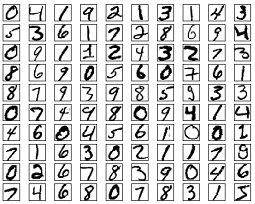
\includegraphics{mnist_100_digits.png}
\caption{Part of the so-called MNIST training sample}
\end{figure}

By increasing the number of training examples, the network can learn
more about handwriting, and so improve its accuracy. So while I've shown
just 100 training digits above, we could certainly build a better
handwriting recognizer by using thousands or even millions or billions
of training examples (\textbf{as we have seen above neural nets are not
capable of extrapolating results, hence it won't recongnize a digit
written in some strange way not included in the training sample !!!}).

Let's try to implement an ANN that is capable of recognizing handwritten
digits. To start we need to install another module, \texttt{mnist} which
containes various predefined training samples. This can be done by using
\texttt{pip}, which is a very useful tool that allows to install new
modules to your python libraries or alternatively using the Anaconda GUI
following the \emph{Environment} tab.

Our program will be based on a Convolutional Neural Network (CNN) which
is specifically designed for image/pattern recognition. We won't go in
the details since it is outside the scope of this lecture but it works
essentially by applying on top of an image a series of filters
(\emph{convolutional layers}) that works as edge detectors and with them
it classifies the images according to their relevant features.

Convolutional layers prove very effective, and stacking them in deep
models allows layers close to the input to learn low-level features
(e.g.~lines) and layers deeper in the model to learn high-order or more
abstract features, like shapes or specific objects.

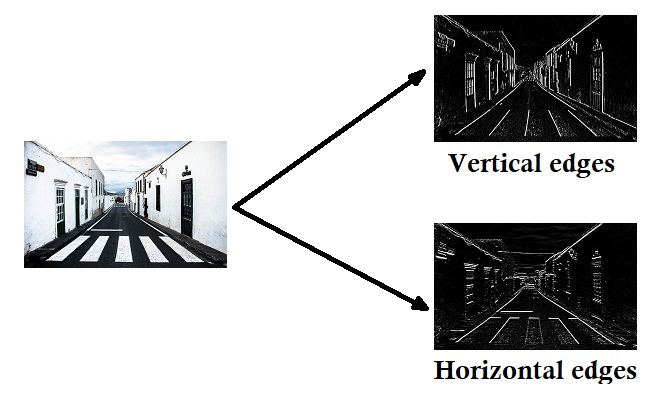
\includegraphics{edges.jpg}

Another important difference with respect to the previous examples is
that in this case we are going to solve a classification problem
(contrary to before when we were trying to regress a sample or in other
word to approximate a function). Indeed our NN output won't be a single
number but rather a vector containing the probabilties that a
handwritten digit was 0, 1, 2, \ldots{}, 8 and 9.

    \begin{tcolorbox}[breakable, size=fbox, boxrule=1pt, pad at break*=1mm,colback=cellbackground, colframe=cellborder]
\begin{Verbatim}[commandchars=\\\{\}]
\PY{k+kn}{import} \PY{n+nn}{numpy} \PY{k}{as} \PY{n+nn}{np}
\PY{c+c1}{\PYZsh{} contains our dataset for training}
\PY{k+kn}{import} \PY{n+nn}{mnist} 

\PY{k+kn}{from} \PY{n+nn}{finnn} \PY{k}{import} \PY{n}{FinNN}

\PY{c+c1}{\PYZsh{} load the training}
\PY{n}{train\PYZus{}images} \PY{o}{=} \PY{n}{mnist}\PY{o}{.}\PY{n}{train\PYZus{}images}\PY{p}{(}\PY{p}{)} \PY{c+c1}{\PYZsh{} the actual images}
\PY{n}{train\PYZus{}labels} \PY{o}{=} \PY{n}{mnist}\PY{o}{.}\PY{n}{train\PYZus{}labels}\PY{p}{(}\PY{p}{)} \PY{c+c1}{\PYZsh{} the truth (it is a 0, 1, 2...)}

\PY{c+c1}{\PYZsh{} 0 means do not split the sample in training and testing sets}
\PY{c+c1}{\PYZsh{} (MNIST has already dont it for us)}
\PY{c+c1}{\PYZsh{} the last parameter tells FinNN class that we are going to develop a CNN}
\PY{n}{trainer} \PY{o}{=} \PY{n}{FinNN}\PY{p}{(}\PY{l+s+s2}{\PYZdq{}}\PY{l+s+s2}{CNN2D}\PY{l+s+s2}{\PYZdq{}}\PY{p}{)}
\PY{n}{trainer}\PY{o}{.}\PY{n}{setData}\PY{p}{(}\PY{n}{train\PYZus{}images}\PY{p}{,} \PY{n}{train\PYZus{}labels}\PY{p}{)}

\PY{c+c1}{\PYZsh{}trainer.normalize()}
\PY{c+c1}{\PYZsh{} for technical reasons you need to expand axis}
\PY{n}{trainer}\PY{o}{.}\PY{n}{x} \PY{o}{=} \PY{n}{np}\PY{o}{.}\PY{n}{expand\PYZus{}dims}\PY{p}{(}\PY{n}{trainer}\PY{o}{.}\PY{n}{x}\PY{p}{,} \PY{n}{axis}\PY{o}{=}\PY{l+m+mi}{3}\PY{p}{)}
\end{Verbatim}
\end{tcolorbox}

    Next we define the CNN architecture.

    \begin{tcolorbox}[breakable, size=fbox, boxrule=1pt, pad at break*=1mm,colback=cellbackground, colframe=cellborder]
\prompt{In}{incolor}{11}{\boxspacing}
\begin{Verbatim}[commandchars=\\\{\}]
\PY{c+c1}{\PYZsh{} define our convolutional NN}
\PY{c+c1}{\PYZsh{} we decide to apply 8 filters to the images }
\PY{c+c1}{\PYZsh{} each with 3x3 pixels size}
\PY{c+c1}{\PYZsh{} the input images have 28x28 pixels size instead}
\PY{n}{trainer}\PY{o}{.}\PY{n}{addConv2DLayer}\PY{p}{(}\PY{l+m+mi}{8}\PY{p}{,} \PY{l+m+mi}{3}\PY{p}{,} \PY{p}{(}\PY{l+m+mi}{28}\PY{p}{,} \PY{l+m+mi}{28}\PY{p}{,} \PY{l+m+mi}{1}\PY{p}{)}\PY{p}{)}

\PY{c+c1}{\PYZsh{} the output is given by 10 neurons returning the }
\PY{c+c1}{\PYZsh{} probability that image is in each class.}
\PY{n}{trainer}\PY{o}{.}\PY{n}{addCNNOutputLayer}\PY{p}{(}\PY{l+m+mi}{10}\PY{p}{)}
        

\PY{c+c1}{\PYZsh{} adam is an algorithm to adjust the weights every cycle}
\PY{c+c1}{\PYZsh{} loss function compute the error between the prediction and the truth }
\PY{c+c1}{\PYZsh{} metrics which error to use }
\PY{n}{trainer}\PY{o}{.}\PY{n}{compileModel}\PY{p}{(}\PY{l+s+s1}{\PYZsq{}}\PY{l+s+s1}{categorical\PYZus{}crossentropy}\PY{l+s+s1}{\PYZsq{}}\PY{p}{,} \PY{l+s+s1}{\PYZsq{}}\PY{l+s+s1}{adam}\PY{l+s+s1}{\PYZsq{}}\PY{p}{)}

\PY{n}{trainer}\PY{o}{.}\PY{n}{fit}\PY{p}{(}\PY{l+m+mi}{5}\PY{p}{)}
\PY{c+c1}{\PYZsh{}validation\PYZus{}data=(test\PYZus{}images, to\PYZus{}categorical(test\PYZus{}labels)))}
    
\PY{n}{trainer}\PY{o}{.}\PY{n}{saveModel}\PY{p}{(}\PY{l+s+s1}{\PYZsq{}}\PY{l+s+s1}{digit\PYZus{}training}\PY{l+s+s1}{\PYZsq{}}\PY{p}{)}

Epoch 1/5
59999/59999 [==============================] - 11s 179us/step - loss: 1.8219
Epoch 2/5
59999/59999 [==============================] - 11s 179us/step - loss: 0.4252
Epoch 3/5
59999/59999 [==============================] - 11s 178us/step - loss: 0.2709
Epoch 4/5
59999/59999 [==============================] - 11s 178us/step - loss: 0.2130
Epoch 5/5
59999/59999 [==============================] - 11s 179us/step - loss: 0.1846
    \end{Verbatim}
\end{tcolorbox}


 \subsubsection{For the most curious
students}\label{for-the-most-curious-students}

If you look closely to the \texttt{finnn.py} module you will notice that
I have cheated when describing the CNN architecture. In particular I
have not mentioned the \texttt{MaxPooling2D} layer, so let's clarify its
feature.

Convolutional layers in a convolutional neural network systematically
apply learned filters to input images in order to create feature maps
that summarize the presence of those features in the input.

A limitation of the feature map output of convolutional layers is that
they record the precise position of features in the input. This means
that small movements in the position of the feature in the input image
will result in a different feature map. This can happen with
re-cropping, rotation, shifting, and other minor changes to the input
image.

Imagine a program that look for car plates in pictures taken by a speed
radar, cars won't be in the same position in the frame so there may be
differences in the classification of similar (but not equal) pictures.

A common approach to address this problem from signal processing is
called \emph{down sampling}. This is where a lower resolution version of
an input signal (e.g.~the picture) is created that still contains the
large or important structural elements, without the fine detail that may
not be as useful to the task.

Down sampling can be achieved using a pooling layer.

Pooling involves selecting a pooling operation, much like a filter to be
applied to feature maps. The size of the pooling operation or filter is
smaller than the size of the feature map; specifically, it is almost
always 2×2 pixels. This means that the pooling layer will always reduce
the size of each feature map by a factor of 2, e.g.~each dimension is
halved. For example, a pooling layer applied to a feature map of 6×6 (36
pixels) will result in an output pooled feature map of 3×3 (9 pixels).

The most common pooling operation are: * Average Pooling: calculate the
average value for each patch on the feature map; * Maximum Pooling (or
Max Pooling): calculate the maximum value for each patch of the feature
map.

Now let's try to see how well our NN predicts MNIST testing digits.

    \begin{tcolorbox}[breakable, size=fbox, boxrule=1pt, pad at break*=1mm,colback=cellbackground, colframe=cellborder]
\begin{Verbatim}[commandchars=\\\{\}]
\PY{k+kn}{import} \PY{n+nn}{numpy} \PY{k}{as} \PY{n+nn}{np}
\PY{k+kn}{import} \PY{n+nn}{mnist}

\PY{n}{trainer}\PY{o}{.}\PY{n}{loadModel}\PY{p}{(}\PY{l+s+s1}{\PYZsq{}}\PY{l+s+s1}{digit\PYZus{}training}\PY{l+s+s1}{\PYZsq{}}\PY{p}{)}

\PY{c+c1}{\PYZsh{} testing with mnist test sample}
\PY{n}{test\PYZus{}images} \PY{o}{=} \PY{n}{mnist}\PY{o}{.}\PY{n}{test\PYZus{}images}\PY{p}{(}\PY{p}{)}
\PY{n}{test\PYZus{}labels} \PY{o}{=} \PY{n}{mnist}\PY{o}{.}\PY{n}{test\PYZus{}labels}\PY{p}{(}\PY{p}{)}

\PY{n}{test\PYZus{}images} \PY{o}{=} \PY{n}{np}\PY{o}{.}\PY{n}{expand\PYZus{}dims}\PY{p}{(}\PY{n}{test\PYZus{}images}\PY{p}{,} \PY{n}{axis}\PY{o}{=}\PY{l+m+mi}{3}\PY{p}{)}

\PY{n}{predictions} \PY{o}{=} \PY{n}{trainer}\PY{o}{.}\PY{n}{predict}\PY{p}{(}\PY{n}{test\PYZus{}images}\PY{p}{[}\PY{p}{:}\PY{l+m+mi}{10}\PY{p}{]}\PY{p}{)}
\PY{n+nb}{print} \PY{p}{(}\PY{l+s+s2}{\PYZdq{}}\PY{l+s+s2}{Tesing on MNIST digits...}\PY{l+s+s2}{\PYZdq{}}\PY{p}{)}
\PY{n+nb}{print}\PY{p}{(}\PY{l+s+s2}{\PYZdq{}}\PY{l+s+s2}{Predicted: }\PY{l+s+s2}{\PYZdq{}}\PY{p}{,} \PY{n}{np}\PY{o}{.}\PY{n}{argmax}\PY{p}{(}\PY{n}{predictions}\PY{p}{,} \PY{n}{axis}\PY{o}{=}\PY{l+m+mi}{1}\PY{p}{)}\PY{p}{)} 
\PY{n+nb}{print}\PY{p}{(}\PY{l+s+s2}{\PYZdq{}}\PY{l+s+s2}{Truth:}\PY{l+s+s2}{\PYZdq{}}\PY{p}{,} \PY{n}{test\PYZus{}labels}\PY{p}{[}\PY{p}{:}\PY{l+m+mi}{10}\PY{p}{]}\PY{p}{)}

\PY{c+c1}{\PYZsh{} this line returns the highest probability of the vector}
\PY{n+nb}{print}\PY{p}{(}\PY{l+s+s2}{\PYZdq{}}\PY{l+s+s2}{highest prob.:}\PY{l+s+s2}{\PYZdq{}}\PY{p}{,} \PY{p}{[}\PY{l+s+s2}{\PYZdq{}}\PY{l+s+si}{\PYZob{}:.6f\PYZcb{}}\PY{l+s+s2}{\PYZdq{}}\PY{o}{.}\PY{n}{format}\PY{p}{(}\PY{n}{p}\PY{p}{[}\PY{n}{np}\PY{o}{.}\PY{n}{argmax}\PY{p}{(}\PY{n}{p}\PY{p}{)}\PY{p}{]}\PY{p}{)} \PY{k}{for} \PY{n}{p} \PY{o+ow}{in} \PY{n}{predictions}\PY{p}{]}\PY{p}{)}

Testing on MNIST digits{\ldots}
Predicted:  [7 2 1 0 4 1 4 9 6 9]
Truth: [7 2 1 0 4 1 4 9 5 9]
highest prob.: ['1.000000', '1.000000', '0.999987', '0.999998', '1.000000',
'0.999993', '0.993805', '0.652628', '0.959723', '0.999988']
    \end{Verbatim}
\end{tcolorbox}

    Since the last two digits have lower probabilities let's check the entire
vectors to see which other number have non-zero probability.

    \begin{tcolorbox}[breakable, size=fbox, boxrule=1pt, pad at break*=1mm,colback=cellbackground, colframe=cellborder]
\begin{Verbatim}[commandchars=\\\{\}]
\PY{n+nb}{print}\PY{p}{(}\PY{l+s+s2}{\PYZdq{}}\PY{l+s+s2}{8th digit:}\PY{l+s+s2}{\PYZdq{}}\PY{p}{,} \PY{p}{[}\PY{l+s+s2}{\PYZdq{}}\PY{l+s+s2}{dig }\PY{l+s+si}{\PYZob{}\PYZcb{}}\PY{l+s+s2}{: }\PY{l+s+si}{\PYZob{}:.6f\PYZcb{}}\PY{l+s+s2}{\PYZdq{}}\PY{o}{.}\PY{n}{format}\PY{p}{(}\PY{n}{i}\PY{p}{,} \PY{n}{p}\PY{p}{)} \PY{k}{for} \PY{n}{i}\PY{p}{,} \PY{n}{p} \PY{o+ow}{in} \PY{n+nb}{enumerate}\PY{p}{(}\PY{n}{predictions}\PY{p}{[}\PY{l+m+mi}{7}\PY{p}{]}\PY{p}{)}\PY{p}{]}\PY{p}{)}
\PY{n+nb}{print} \PY{p}{(}\PY{p}{)}
\PY{n+nb}{print}\PY{p}{(}\PY{l+s+s2}{\PYZdq{}}\PY{l+s+s2}{9th digit:}\PY{l+s+s2}{\PYZdq{}}\PY{p}{,} \PY{p}{[}\PY{l+s+s2}{\PYZdq{}}\PY{l+s+s2}{dig }\PY{l+s+si}{\PYZob{}\PYZcb{}}\PY{l+s+s2}{: }\PY{l+s+si}{\PYZob{}:.6f\PYZcb{}}\PY{l+s+s2}{\PYZdq{}}\PY{o}{.}\PY{n}{format}\PY{p}{(}\PY{n}{i}\PY{p}{,} \PY{n}{p}\PY{p}{)} \PY{k}{for} \PY{n}{i}\PY{p}{,} \PY{n}{p} \PY{o+ow}{in} \PY{n+nb}{enumerate}\PY{p}{(}\PY{n}{predictions}\PY{p}{[}\PY{l+m+mi}{8}\PY{p}{]}\PY{p}{)}\PY{p}{]}\PY{p}{)}

8th digit: ['dig 0: 0.000000', 'dig 1: 0.000000', 'dig 2: 0.000232', 'dig 3:
0.000034', 'dig 4: 0.347104', 'dig 5: 0.000001', 'dig 6: 0.000000', 'dig 7:
0.000001', 'dig 8: 0.000000', 'dig 9: 0.652628']

9th digit: ['dig 0: 0.000000', 'dig 1: 0.000000', 'dig 2: 0.000000', 'dig 3:
0.000000', 'dig 4: 0.000000', 'dig 5: 0.040277', 'dig 6: 0.959723', 'dig 7:
0.000000', 'dig 8: 0.000000', 'dig 9: 0.000000']
    \end{Verbatim}
\end{tcolorbox}

    So in the first case the second ranked digit is 5 (which can be confused
with a six if the lower loop is almost closed), while in the second case
it is a 7 (which can be confused with a 9 if the loop is opened).

\subsubsection{Exercise 8.2}\label{exercise-8.2}

To see how well our NN behaves with different kind of digits we will try
to check how it works with my calligraphy (as homework try to repeat the
exercise using your own digit following the instructions given below).

\begin{itemize}
\tightlist
\item
  Open \texttt{paint} and create a 280x280 white square
\item
  Change brush type and set the maximum size
\item
  With the mouse draw a digit
\item
  Finally save the file (e.g.~five.png)
\end{itemize}

Before passing the image to the NN it has to be resized and this is done
with an ad-hoc function (\texttt{transform\_image}) which is in the
\texttt{digit\_converter.py} module.

    \begin{tcolorbox}[breakable, size=fbox, boxrule=1pt, pad at break*=1mm,colback=cellbackground, colframe=cellborder]
\begin{Verbatim}[commandchars=\\\{\}]
\PY{k+kn}{from} \PY{n+nn}{digit\PYZus{}converter} \PY{k}{import} \PY{n}{transform\PYZus{}image}

\PY{n}{filenames} \PY{o}{=} \PY{p}{[}\PY{l+s+s1}{\PYZsq{}}\PY{l+s+s1}{four.png}\PY{l+s+s1}{\PYZsq{}}\PY{p}{,} \PY{l+s+s1}{\PYZsq{}}\PY{l+s+s1}{five.png}\PY{l+s+s1}{\PYZsq{}}\PY{p}{]}

\PY{k}{for} \PY{n}{f} \PY{o+ow}{in} \PY{n}{filenames}\PY{p}{:}
    \PY{n}{test\PYZus{}images} \PY{o}{=} \PY{n}{np}\PY{o}{.}\PY{n}{array}\PY{p}{(}\PY{n}{transform\PYZus{}image}\PY{p}{(}\PY{n}{f}\PY{p}{)}\PY{p}{)}
    \PY{n}{test\PYZus{}images} \PY{o}{=} \PY{n}{np}\PY{o}{.}\PY{n}{expand\PYZus{}dims}\PY{p}{(}\PY{n}{test\PYZus{}images}\PY{p}{,} \PY{n}{axis}\PY{o}{=}\PY{l+m+mi}{3}\PY{p}{)}

    \PY{n}{predict} \PY{o}{=} \PY{n}{trainer}\PY{o}{.}\PY{n}{predict}\PY{p}{(}\PY{n}{test\PYZus{}images}\PY{p}{)}
    \PY{n+nb}{print} \PY{p}{(}\PY{l+s+s2}{\PYZdq{}}\PY{l+s+se}{\PYZbs{}n}\PY{l+s+s2}{\PYZdq{}}\PY{p}{)}
    \PY{n+nb}{print} \PY{p}{(}\PY{l+s+s2}{\PYZdq{}}\PY{l+s+s2}{Tesing on custom digits...}\PY{l+s+s2}{\PYZdq{}}\PY{p}{)}
    \PY{n+nb}{print} \PY{p}{(}\PY{l+s+s2}{\PYZdq{}}\PY{l+s+s2}{Predicted: }\PY{l+s+s2}{\PYZdq{}}\PY{p}{,} \PY{n}{np}\PY{o}{.}\PY{n}{argmax}\PY{p}{(}\PY{n}{predict}\PY{p}{,} \PY{n}{axis}\PY{o}{=}\PY{l+m+mi}{1}\PY{p}{)}\PY{p}{)}
    \PY{n+nb}{print}\PY{p}{(}\PY{l+s+s2}{\PYZdq{}}\PY{l+s+s2}{\PYZpc{}}\PY{l+s+s2}{:}\PY{l+s+s2}{\PYZdq{}}\PY{p}{,} \PY{p}{[}\PY{l+s+s2}{\PYZdq{}}\PY{l+s+si}{\PYZob{}:.3f\PYZcb{}}\PY{l+s+s2}{\PYZdq{}}\PY{o}{.}\PY{n}{format}\PY{p}{(}\PY{n}{p}\PY{p}{[}\PY{n}{np}\PY{o}{.}\PY{n}{argmax}\PY{p}{(}\PY{n}{p}\PY{p}{)}\PY{p}{]}\PY{p}{)} \PY{k}{for} \PY{n}{p} \PY{o+ow}{in} \PY{n}{predict}\PY{p}{]}\PY{p}{)}
      
Testing on custom digits{\ldots}
Predicted:  [4]
\%: ['1.000']

Testing on custom digits{\ldots}
Predicted:  [5]
\%: ['0.999']
    \end{Verbatim}
\end{tcolorbox}

Those the images I have checked:

\begin{figure}
  \centering
  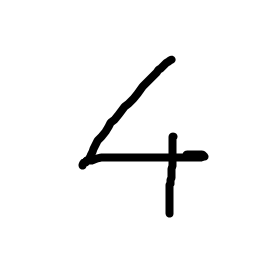
\includegraphics[width=0.2\linewidth]{four.png}
  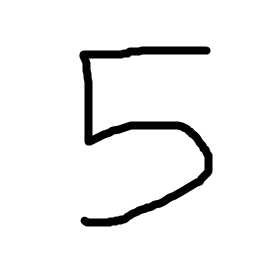
\includegraphics[width=0.2\linewidth]{five.png}
\end{figure}

\section{Technical Analysis}\label{technical-analysis}

In finance, \emph{technical analysis} is a security analysis discipline
for forecasting the direction of prices through the study of past market
data, primarily price and volume. Essentially the analyst looks for
particular patterns in the price time series that are \emph{known} to
develop in predictable ways to take profit of it.

\begin{figure}
  \centering
  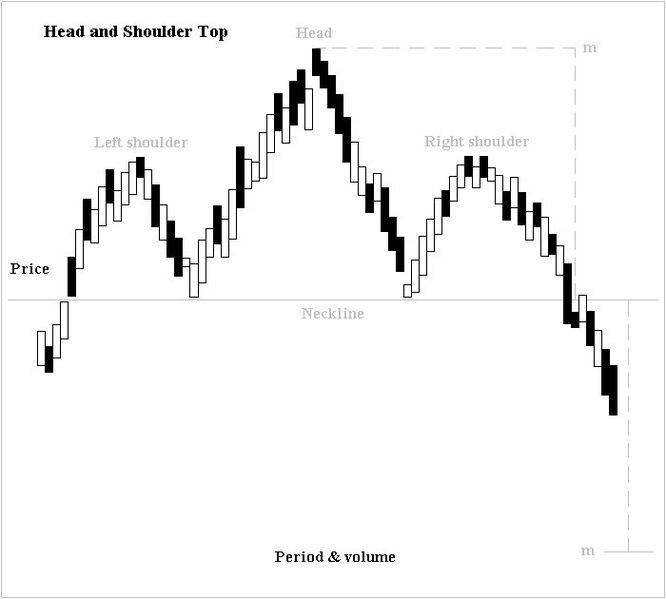
\includegraphics[width=0.4\linewidth]{H_and_s_top_new.jpg}
  
  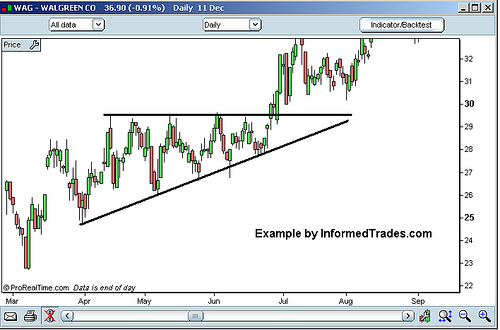
\includegraphics[width=0.4\linewidth]{Triangle-ascending.jpg}
  \caption{Examples of patterns in real time series.}
\end{figure}

As you may imagine we will try to develop a CNN (like in the handwriting
case) capable of classifying features in time series to be used in a
technical analysis (this is much faster than having somebody looking at
thousands of time series by eye\ldots{}).

I have generated myself the training set simulating 21600 time series
(1/3 with head and shoulder patter, 1/3 with triangle pattern and 1/3
with no pattern). \emph{To make the training easier the features have
been exagerated.}

\begin{figure}
  \centering
  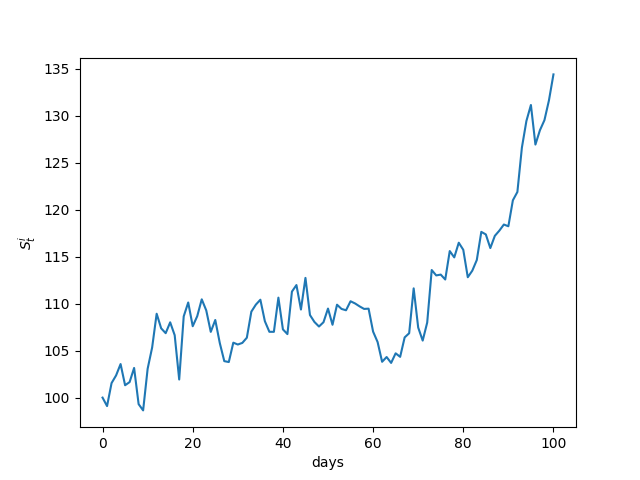
\includegraphics[width=0.6\linewidth]{image_1.png}
  \caption{An example of training image with no pattern.}
\end{figure}

\begin{figure}
  \centering
  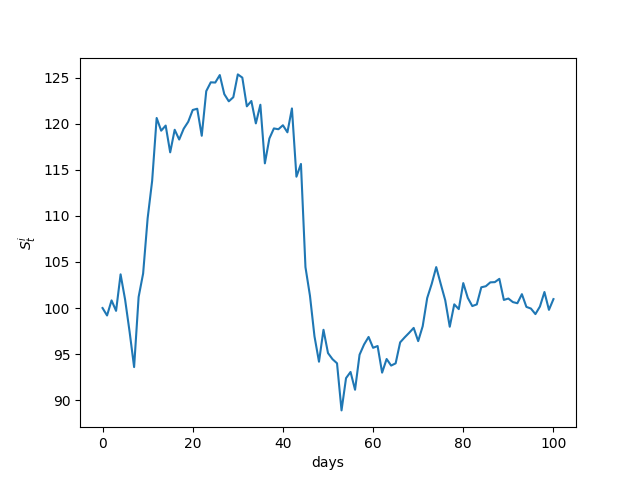
\includegraphics[width=0.6\linewidth]{image_2.png}
  \caption{An example of training image with \emph{head and shoulder} pattern.}
\end{figure}

\begin{figure}
  \centering
  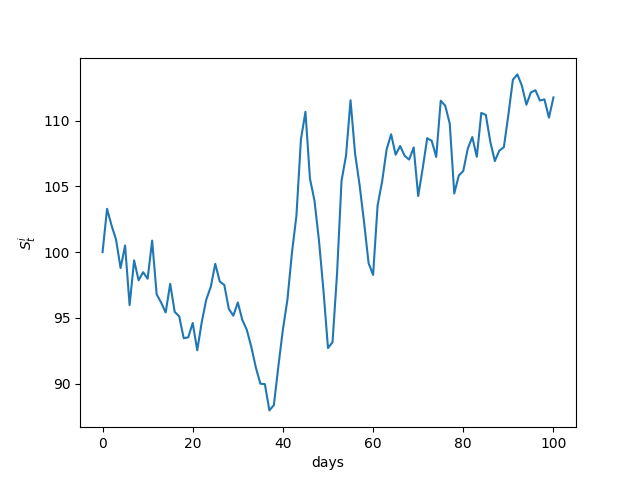
\includegraphics[width=0.6\linewidth]{image_0.png}
  \caption{An example of training image with \emph{triangle} pattern.}
\end{figure}

    \begin{tcolorbox}[breakable, size=fbox, boxrule=1pt, pad at break*=1mm,colback=cellbackground, colframe=cellborder]
\begin{Verbatim}[commandchars=\\\{\}]
\PY{k+kn}{from} \PY{n+nn}{finnn} \PY{k}{import} \PY{n}{FinNN}
\PY{k+kn}{import} \PY{n+nn}{pandas} \PY{k}{as} \PY{n+nn}{pd}
\PY{k+kn}{import} \PY{n+nn}{numpy} \PY{k}{as} \PY{n+nn}{np}

\PY{n}{train\PYZus{}labels} \PY{o}{=} \PY{n}{pd}\PY{o}{.}\PY{n}{read\PYZus{}csv}\PY{p}{(}\PY{l+s+s2}{\PYZdq{}}\PY{l+s+s2}{training\PYZus{}techana\PYZus{}labels.csv}\PY{l+s+s2}{\PYZdq{}}\PY{p}{)}
\PY{n}{train\PYZus{}images} \PY{o}{=} \PY{n}{pd}\PY{o}{.}\PY{n}{read\PYZus{}csv}\PY{p}{(}\PY{l+s+s2}{\PYZdq{}}\PY{l+s+s2}{training\PYZus{}techana\PYZus{}images.csv}\PY{l+s+s2}{\PYZdq{}}\PY{p}{)}
\PY{c+c1}{\PYZsh{}train\PYZus{}images = train\PYZus{}images[:3000]}
\PY{c+c1}{\PYZsh{}train\PYZus{}images = np.array(train\PYZus{}images)}
\PY{n}{train\PYZus{}images} \PY{o}{=} \PY{n}{np}\PY{o}{.}\PY{n}{expand\PYZus{}dims}\PY{p}{(}\PY{n}{train\PYZus{}images}\PY{p}{,} \PY{n}{axis}\PY{o}{=}\PY{l+m+mi}{2}\PY{p}{)}

\PY{n}{trainer} \PY{o}{=} \PY{n}{FinNN}\PY{p}{(}\PY{l+s+s2}{\PYZdq{}}\PY{l+s+s2}{CNN1D}\PY{l+s+s2}{\PYZdq{}}\PY{p}{)}
\PY{n}{trainer}\PY{o}{.}\PY{n}{setData}\PY{p}{(}\PY{n}{train\PYZus{}images}\PY{p}{,} \PY{n}{train\PYZus{}labels}\PY{p}{)}

\PY{c+c1}{\PYZsh{} define the CNN }
\PY{n}{trainer}\PY{o}{.}\PY{n}{addConv1DInputLayer}\PY{p}{(}\PY{l+m+mi}{80}\PY{p}{,} \PY{l+m+mi}{20}\PY{p}{,} \PY{p}{(}\PY{l+m+mi}{101}\PY{p}{,} \PY{l+m+mi}{1}\PY{p}{)}\PY{p}{)}
\PY{n}{trainer}\PY{o}{.}\PY{n}{addConv1DLayer}\PY{p}{(}\PY{l+m+mi}{80}\PY{p}{,} \PY{l+m+mi}{15}\PY{p}{)}
\PY{n}{trainer}\PY{o}{.}\PY{n}{addMaxPooling1D}\PY{p}{(}\PY{l+m+mi}{3}\PY{p}{)}
\PY{n}{trainer}\PY{o}{.}\PY{n}{addConv1DLayer}\PY{p}{(}\PY{l+m+mi}{100}\PY{p}{,} \PY{l+m+mi}{10}\PY{p}{)}
\PY{n}{trainer}\PY{o}{.}\PY{n}{addConv1DLayer}\PY{p}{(}\PY{l+m+mi}{100}\PY{p}{,} \PY{l+m+mi}{5}\PY{p}{)}
\PY{n}{trainer}\PY{o}{.}\PY{n}{addGlobalAveragePooling1D}\PY{p}{(}\PY{p}{)}
\PY{n}{trainer}\PY{o}{.}\PY{n}{addDropout}\PY{p}{(}\PY{l+m+mf}{0.5}\PY{p}{)}
\PY{n}{trainer}\PY{o}{.}\PY{n}{addCNNOutputLayer}\PY{p}{(}\PY{l+m+mi}{3}\PY{p}{)}

\PY{n}{trainer}\PY{o}{.}\PY{n}{compileModel}\PY{p}{(}\PY{l+s+s1}{\PYZsq{}}\PY{l+s+s1}{categorical\PYZus{}crossentropy}\PY{l+s+s1}{\PYZsq{}}\PY{p}{,} \PY{l+s+s1}{\PYZsq{}}\PY{l+s+s1}{adam}\PY{l+s+s1}{\PYZsq{}}\PY{p}{)}

\PY{c+c1}{\PYZsh{} make the training}
\PY{n}{trainer}\PY{o}{.}\PY{n}{fit}\PY{p}{(}\PY{l+m+mi}{80}\PY{p}{,} \PY{l+m+mi}{35}\PY{p}{)}

\PY{n}{trainer}\PY{o}{.}\PY{n}{saveModel}\PY{p}{(}\PY{l+s+s1}{\PYZsq{}}\PY{l+s+s1}{techana}\PY{l+s+s1}{\PYZsq{}}\PY{p}{)}

Epoch 1/80
21598/21598 [==============================] - 17s 774us/step - loss: 0.8423
...
Epoch 80/80
21598/21598 [==============================] - 17s 804us/step - loss: 0.1881
    \end{Verbatim}
\end{tcolorbox}

\subsubsection{Again for the most curious
students}\label{again-for-the-most-curious-students}

Large neural nets trained on relatively small datasets can overfit the
training data.

This has the effect of the model learning the statistical noise in the
training data, which results in poor performance when the model is
evaluated on new data, e.g.~a test dataset.

One approach to reduce overfitting is to fit all possible different
neural networks on the same dataset and to average the predictions from
each model. This is not feasible in practice, and can be approximated
using a small collection of different models, called an ensemble. A
problem even with the ensemble approximation is that it requires
multiple models to be fit and stored, which can be a challenge if the
models are large, requiring days or weeks to train and tune.

\emph{Dropout} is a regularization method that approximates training a
large number of neural networks with different architectures in
parallel.

During training, some number of layer outputs are randomly ignored or
\emph{dropped out}. This has the effect of making the layer look-like
and be treated-like a layer with a different number of nodes and
connectivity to the prior layer. In effect, each update to a layer
during training is performed with a different ``view'' of the configured
layer.

Even if the it may seems counterintuitive (better training when
switching off nodes) indeed dropout breaks-up situations where network
layers co-adapt to correct mistakes from prior layers, in turn making
the model more robust.

To test the performance I wanted to simulate a real case scenario where
the time series are analyzed in real-time in order to predict as soon as
possible a particular pattern and take advantage of the prediction.

To do so I have created a longer time series and passed as input to the
CNN sliding time windows to simulate the evolution of the time series.
The goal was to check when the neural network was capable of predicting
the incoming pattern.

    \begin{tcolorbox}[breakable, size=fbox, boxrule=1pt, pad at break*=1mm,colback=cellbackground, colframe=cellborder]
\begin{Verbatim}[commandchars=\\\{\}]
\PY{k+kn}{import} \PY{n+nn}{numpy} \PY{k}{as} \PY{n+nn}{np}
\PY{k+kn}{import} \PY{n+nn}{csv}
\PY{k+kn}{from} \PY{n+nn}{keras}\PY{n+nn}{.}\PY{n+nn}{models} \PY{k}{import} \PY{n}{Sequential}\PY{p}{,} \PY{n}{load\PYZus{}model}
\PY{k+kn}{from} \PY{n+nn}{keras}\PY{n+nn}{.}\PY{n+nn}{utils} \PY{k}{import} \PY{n}{to\PYZus{}categorical}

\PY{n}{test\PYZus{}images} \PY{o}{=} \PY{n}{pd}\PY{o}{.}\PY{n}{read\PYZus{}csv}\PY{p}{(}\PY{l+s+s2}{\PYZdq{}}\PY{l+s+s2}{testing\PYZus{}techana\PYZus{}frames.csv}\PY{l+s+s2}{\PYZdq{}}\PY{p}{)}
\PY{n}{test\PYZus{}images} \PY{o}{=} \PY{n}{np}\PY{o}{.}\PY{n}{expand\PYZus{}dims}\PY{p}{(}\PY{n}{test\PYZus{}images}\PY{p}{,} \PY{n}{axis}\PY{o}{=}\PY{l+m+mi}{2}\PY{p}{)}

\PY{n}{trainer}\PY{o}{.}\PY{n}{loadModel}\PY{p}{(}\PY{l+s+s1}{\PYZsq{}}\PY{l+s+s1}{techana}\PY{l+s+s1}{\PYZsq{}}\PY{p}{)}

\PY{n}{predictions} \PY{o}{=} \PY{n}{trainer}\PY{o}{.}\PY{n}{predict}\PY{p}{(}\PY{n}{test\PYZus{}images}\PY{p}{)}
\PY{k}{for} \PY{n}{i} \PY{o+ow}{in} \PY{n+nb}{range}\PY{p}{(}\PY{n+nb}{len}\PY{p}{(}\PY{n}{predictions}\PY{p}{)}\PY{p}{)}\PY{p}{:}
    \PY{n+nb}{print} \PY{p}{(}\PY{n}{np}\PY{o}{.}\PY{n}{argmax}\PY{p}{(}\PY{n}{predictions}\PY{p}{[}\PY{n}{i}\PY{p}{]}\PY{p}{)}\PY{p}{,} \PY{p}{[}\PY{l+s+s2}{\PYZdq{}}\PY{l+s+si}{\PYZob{}:.2f\PYZcb{}}\PY{l+s+s2}{\PYZdq{}}\PY{o}{.}\PY{n}{format}\PY{p}{(}\PY{n}{p}\PY{p}{)} \PY{k}{for} \PY{n}{p} \PY{o+ow}{in} \PY{n}{predictions}\PY{p}{[}\PY{n}{i}\PY{p}{]}\PY{p}{]}\PY{p}{)}

0 ['0.71', '0.00', '0.29']
0 ['0.66', '0.00', '0.34']
0 ['0.82', '0.00', '0.18']
0 ['0.91', '0.00', '0.09']
2 ['0.40', '0.06', '0.54']
1 ['0.00', '1.00', '0.00']
1 ['0.00', '1.00', '0.00']
1 ['0.00', '1.00', '0.00']
1 ['0.00', '1.00', '0.00']
    \end{Verbatim}
\end{tcolorbox}

    So at the 6th sample the CNN start recognizing the \emph{head and
shoulder} pattern in the price evolution.
